\documentclass{article}
\usepackage{graphicx} % Required for inserting images
\usepackage[ruled,vlined]{algorithm2e}
\title{SAGA-reSGLD Algorithm}
\author{WILLIAM MAX MORRIS}
\date{August 2025}
\usepackage{parskip}
\usepackage{amsmath}
\usepackage[top=4cm, bottom=4cm]{geometry}
\usepackage[demo]{graphicx}
\usepackage{subfig}
\usepackage[utf8]{inputenc}


\begin{document}

\maketitle

\begin{abstract}
I propose a variance-reduced replica exchange stochastic gradient Langevin dynamics (reSGLD) algorithm based on the SAGA method. 
This approach leverages stored per-sample energy evaluations to reduce gradient noise and provide more stable estimates of energy differences across temperature replicas. 
By incorporating a memory-based correction scheme and an exponential moving average variance estimator, the algorithm improves acceptance probabilities in replica exchange steps and enhances sampling efficiency. 
In this paper, the Algorithm is defined and presented through a toy example.

\end{abstract}
\newpage

\section{Introduction}
The study of Scalable Monte Carlo for Bayesian Learning \cite{Fearnhead2024} 
aims to solve the issues presented when the data set on which we condition is large in size or dimension within our Bayesian framework. These data properties make traditional, exact methods of simulation infeasible. For example, a random walk Metropolis-Hastings algorithm will suffer from poor mixing due to low acceptance rates, and for a Gibbs sampler, high dimensionality often makes the pre-requisite full conditional distributions intractable. More notably, typical reversible Monte Carlo Markov Chain (MCMC) methods suffer from large computational timescales.

Within machine learning, Stochastic Gradient Monte Carlo Markov Chain (SGMCMC) methods accelerate the convergence of optimization problems. Stochastic Gradient Langevin Dynamics (SGLD) \cite{Fearnhead2024} involves constructing a simple estimator for the energy gradient using small subsamples of the data, which, in limit, produces draws from the exact target posterior distribution in question. 

However, this method is limited when presented with multi-modal target distributions, a common occurrence for non-convex optimization problems. The replica exchange SGLD \cite{Deng2021} method takes advantage of our ability to control exploration of the parameter space via the temperature (learning rate). The method explored by Deng et al. utilizes this by sampling two chains in parallel; one with low temperature (for local exploration) and the other with a large temperature (for global exploration). A Metropolis-Hastings step allows tunneling between different modes \cite{Deng2021} however, we must account for the bias introduced by our stochastic gradient estimator by adding a correction factor to the swap rate.

Deng further improved acceleration of convergence of the algorithm \cite{deng2021acceleratingconvergencereplicaexchange} by implementing a control variate method to reduce the variance of our noisy energy estimators; not the gradient estimators.


In this paper I adapt the Variance Reduced replica exchange SGLD (VR-reSGLD) Algorithm by using a SAGA \cite{gower2020variancereducedmethodsmachinelearning} variance reduction which prioritizes computation speed over memory by replacing the global update step with a stored vector of energies $O(Nd)$. Empirically, I test the algorithm on the same gaussian mixture model in Deng et al., 2021 \cite{deng2021acceleratingconvergencereplicaexchange} and provide performance and graph comparisons as well as some considerations throughout.

For practical context, the algorithm is written from scratch in C++ and performance metrics and graphs are evaluated in R (ggplot2 \& coda).

\newpage
\section{The Algorithm}

\begin{algorithm}[H]
\caption{SAGA Variance-Reduced reSGLD with Replica Exchange}
\label{alg:saga-vr-resgld}
\KwIn{Dataset $\{x_i\}_{i=1}^N$, step size $\eta$, minibatch size $n$, 
temperatures $\tau_1, \tau_2$, noise scales $\sigma^{(1)} = \sqrt{2\tau_1 \eta}$, 
$\sigma^{(2)} = \sqrt{2\tau_2 \eta}$, smoothing factor $\alpha$, correction factor $F$}

\textbf{Initialize:} 
parameters $\beta^{(1)},\beta^{(2)} \gets 0$, \\
store per-sample energies $E_i^{(1)} = L(x_i,\beta^{(1)})$, 
$E_i^{(2)} = L(x_i,\beta^{(2)})$, \\
means $\bar{E}^{(1)}, \bar{E}^{(2)}$, \\
variance estimate $\hat{\sigma}^2 \gets 0$.\\

\For{$k=1$ to $K$}
{\textbf{(a) Parallel Sampling :} \\
    Sample minibatch $B \subset \{1,\dots,N\}$ of size $n$. \\
  Update chains by Langevin steps
  \[
    \beta_{(k+1)}^{(h)} \gets \beta_k^{(h)} - \eta \tfrac{N}{n} \sum_{j\in B} \nabla_\beta L(x_j, \beta_h) + \sigma^{(h)} \,\xi^{(h)}, for\ h\in\{1, 2\}
  \]
  where $\xi^{(h)} \sim \mathcal{N}(0,I)$.
  
  \vspace{0.25em}
  \textbf{(b) Variance-reduced energy estimate:} \\
  Using the same minibatch $B$ (or a new smaller batch), compute new energies
  \[
    E_j^{(h,new)} = L(x_j, \beta_h), \quad 
    \Delta_j^{(h)} = E_j^{(h,new)} - E_j^{(h)}.
  \]
  Form unbiased estimators
  \[
    \tilde{L}^{(h)} = \frac{N}{n} \sum_{j \in B} \Delta_j^{(h)} + \bar{E}^{(h)}.
  \]

  \vspace{0.25em}
  \textbf{(c) Update SAGA memory:} \\
  \For{$j \in B$}{
    $E_j^{(h)} \gets E_j^{(h,new)}$ \;
    $\bar{E}^{(h)} \gets \bar{E}^{(h)} + \tfrac{1}N \sum_{j \in B} \Delta_j^{(h)}$.
  }

  
  \vspace{0.25em}
  \textbf{(d) Variance estimation:} \\
  Repeat $K_{\text{var}}$ times: sample minibatch $B'$, form differences 
  $d = \tilde{L}^{(1)} - \tilde{L}^{(2)}$, 
  accumulate empirical variance $\mathrm{Var}[d]$. \\
  Update EMA:
  \[
    \hat{\sigma}^2 \gets (1-\alpha)\hat{\sigma}^2 + \alpha \cdot \mathrm{Var}[d].
  \]
  
  \vspace{0.25em}
  \textbf{(e) Swap step:} \\
  Compute
  \[ S = \min\left\{1, \exp\!\Big( (\frac{1}{\tau_1}-\frac{1}{\tau_2}) \cdot \big[ 
    \tilde{L}^{(1)} - \tilde{L}^{(2)} - (\frac{1}{\tau_1}-\frac{1}{\tau_2})\tfrac{\hat{\sigma}^2}{F} 
    \big]\Big)\right\}.
  \]
  With\ probability\ \ensuremath{S}, swap\ $(\beta_1, \beta_2)$ together with their memory 
  $(E^{(1)},E^{(2)},\bar{E}^{(1)},\bar{E}^{(2)})$.
  
}

\KwOut{Sample path $\{\beta_1^{(k)}\}$ at the cold temperature $\tau_1$.}
\end{algorithm}

\newpage
\section{Experiment - Simulation of Gaussian mixture distribution}

\begin{figure}[t]%
    \centering
    \subfloat[\centering VR-reSGLD output]{{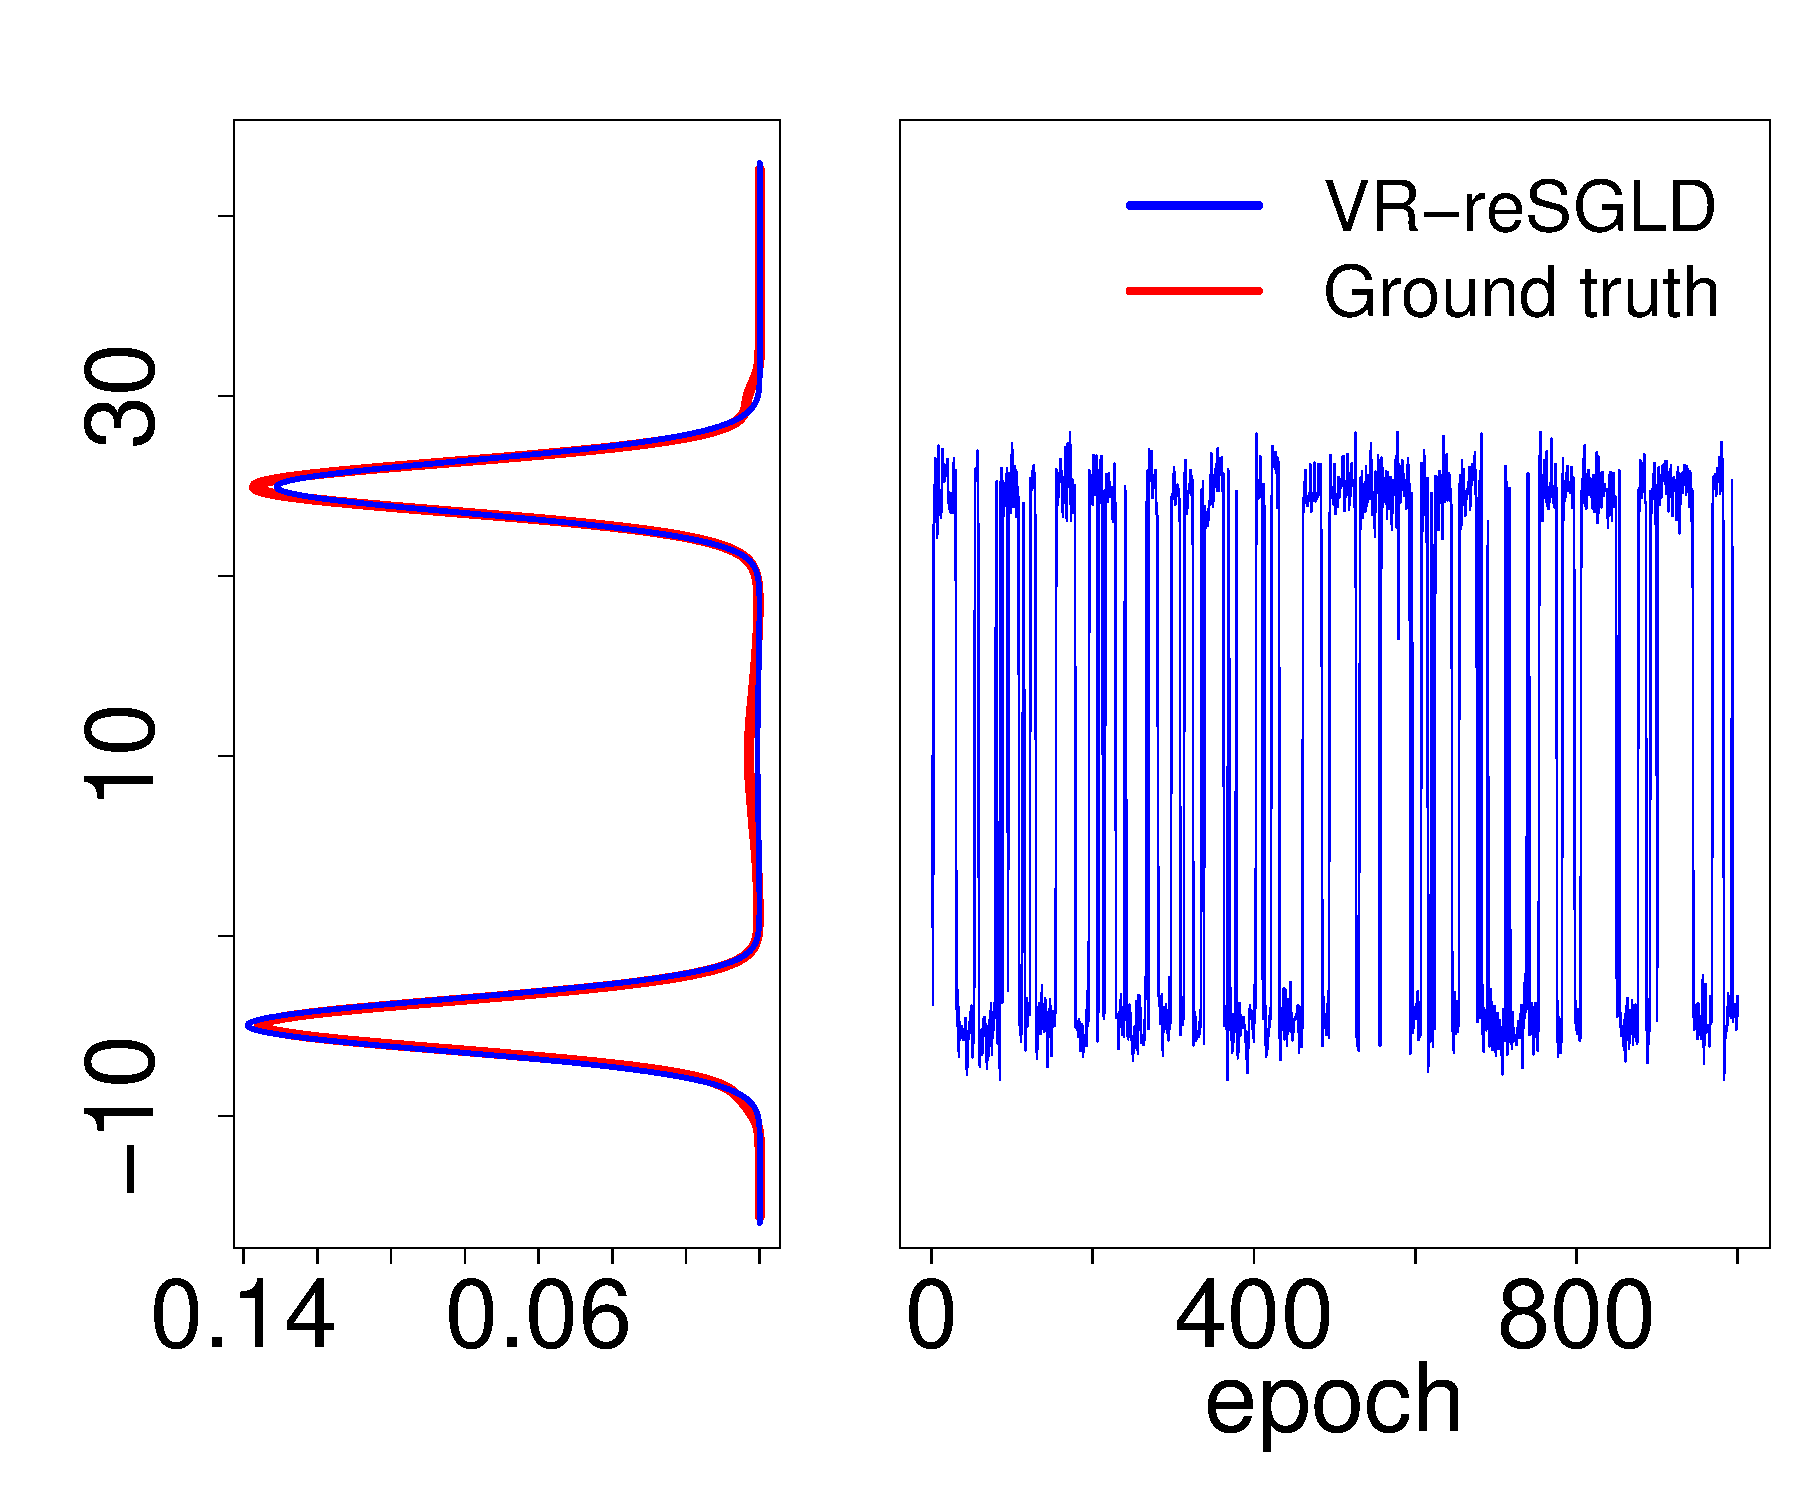
\includegraphics[width=5cm]{wei_trace1.pdf} }}%
    \qquad
    \subfloat[\centering Output of methods previous to Deng et al.]{{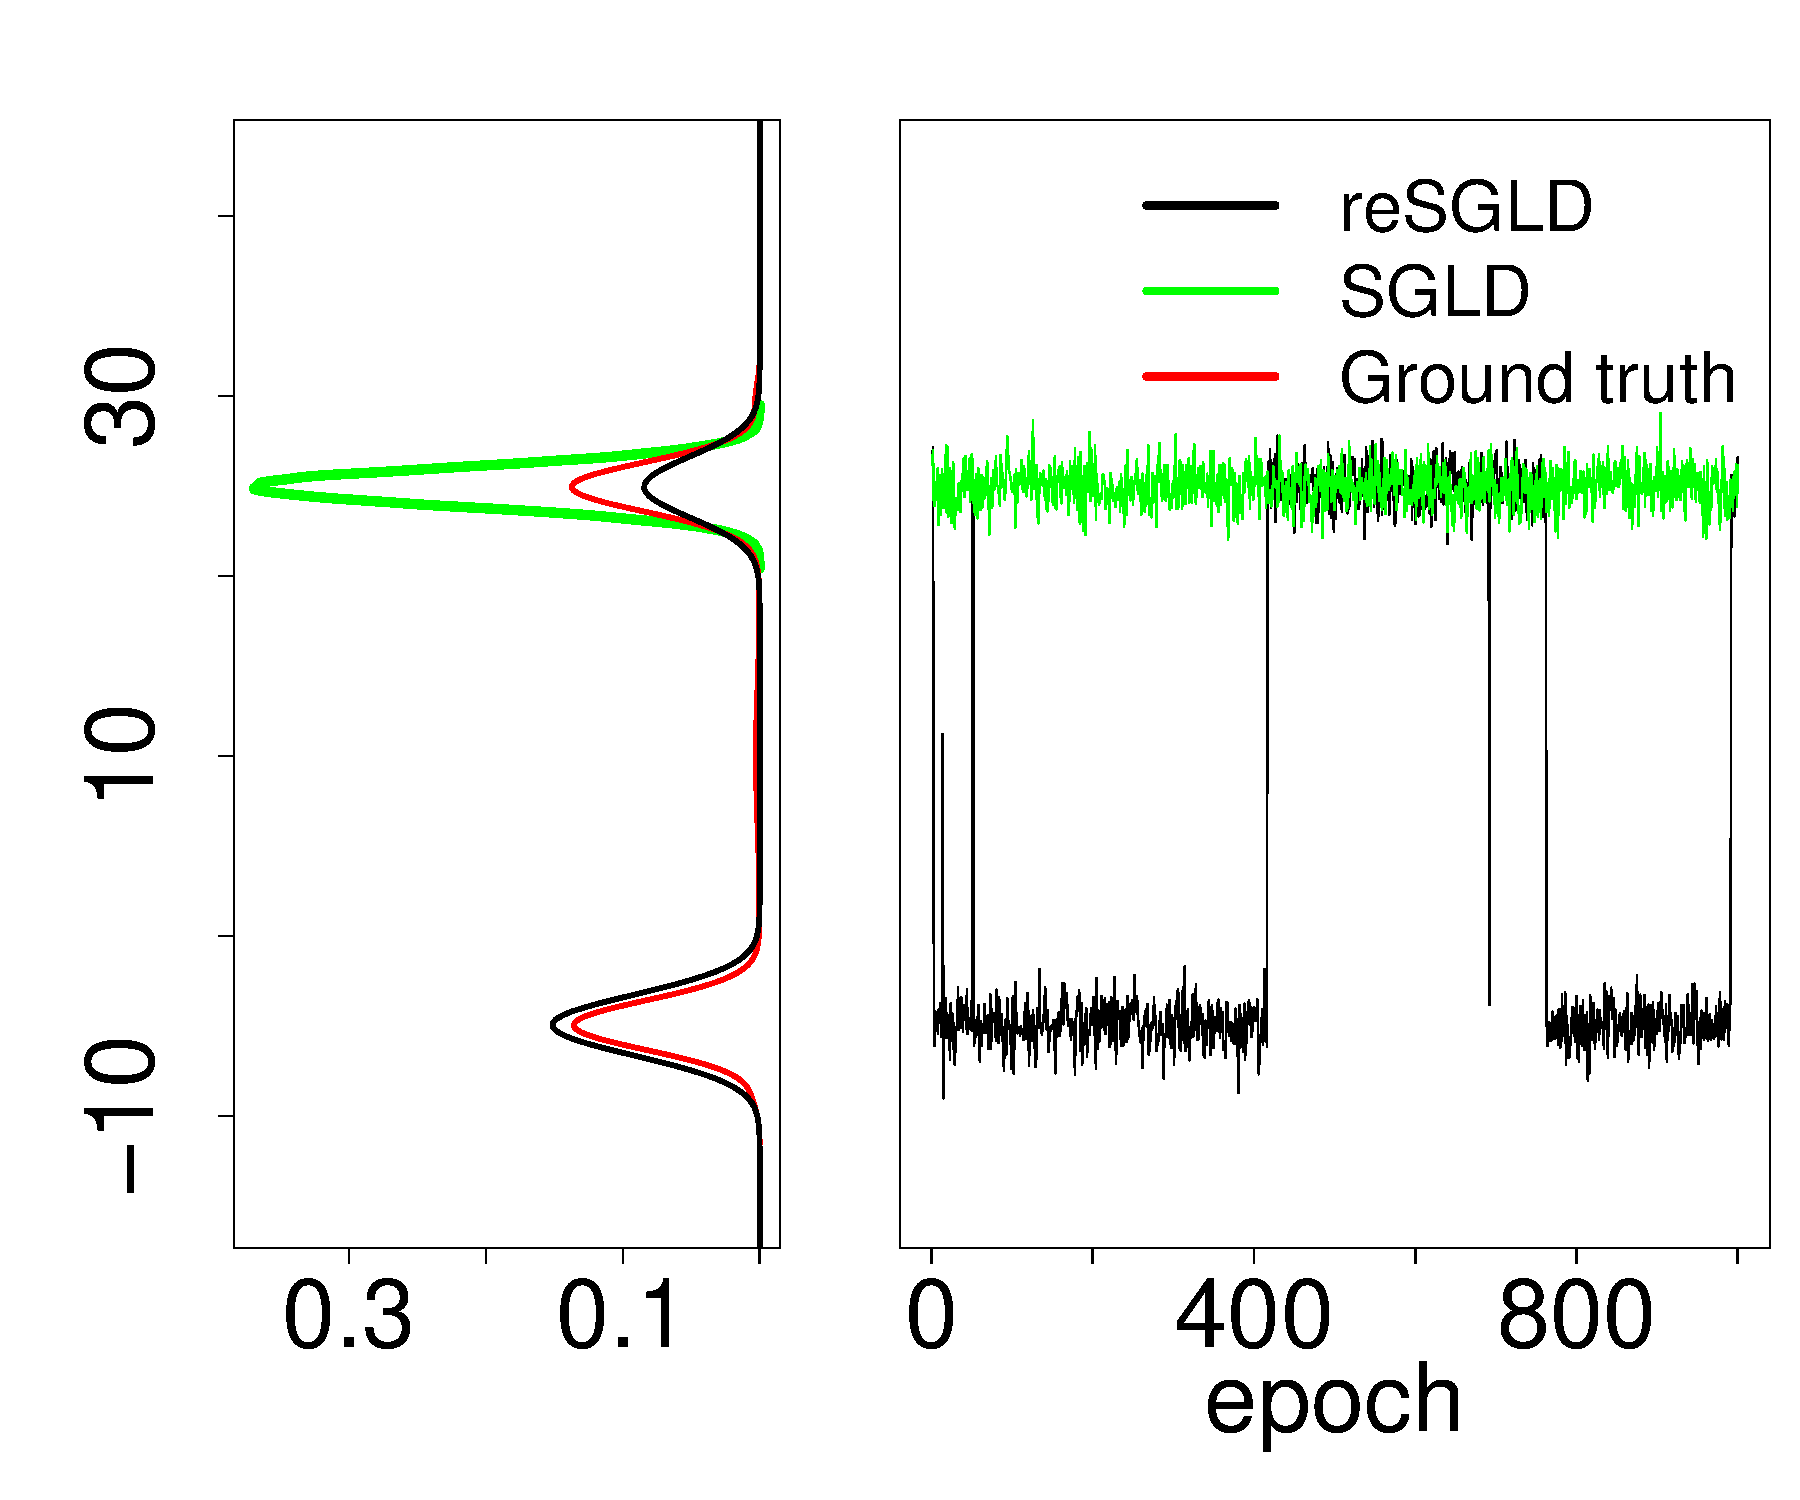
\includegraphics[width=5cm]{Wei_trace2.pdf} }}%
    \caption{Trace plots and KDE's pf $\beta^{(1)}$ for various models of the toy example.}%
    \label{fig:example}%
\end{figure}

We evaluate the SAGA-reSGLD algorithm on a synthetic Gaussian mixture posterior, following the setup from Deng et al. \cite{deng2021acceleratingconvergencereplicaexchange}. Specifically, we assume data generated from a mixture of two Gaussians  $x_i \;\big|\; \beta \;\sim\; 
0.5\,\mathcal{N}(\beta, \sigma^{2}) \;+\; 
0.5\,\mathcal{N}(\phi - \beta, \sigma^{2}),
\text{where } \phi = 20,\; \sigma = 5,\;$ and $\beta$ is set to -5 (apriori).

The target posterior distribution for $\beta$ given the observed $x_i$ is proportional to $f(\beta \ | \ x_{1:N}) \propto \Pi_{i=1}^{N} \ 0.5\,\mathcal{N}(x_i\, ;\,\beta,\,\sigma^2) \; + \; 0.5\,\mathcal{N}(x_i\, ;\,\beta,\,\phi\, -\,\sigma^2)   $.

This posterior is bimodal and non-convex: intuitively, there are two plausible explanations for the data (since swapping $\beta$ with $\phi-\beta$ leaves the mixture likelihood unchanged). The two modes are roughly around the true generating value (near $\beta=-5$) and its symmetric counterpart (around $\beta \approx 25$ given $\phi=20$). Such a scenario poses a challenge for MCMC algorithms, making it an ideal test for assessing mode-switching and mixing efficiency. We compare the performance of our SAGA-reSGLD algorithm with Deng et al.'s VR-reSGLD on this problem.


For a fair comparison,both algorithms were tuned with similar initial hyper-parameters. The VR-reSGLD algorithm was configured with mini-batch size $n = 0.1,N$, where here we use $N = 10,000$, temperatures $(\tau_1, \tau_2) = (10,;1000)$, step size $\eta = 1\times 10^{-7}$, correction factor $F = 1$, and smoothing factor $\alpha = 0.2$. These settings mirror those used in Deng et al. \cite{deng2021acceleratingconvergencereplicaexchange} for the Gaussian mixture example (notably, VR-reSGLD can use a small $F=1$ because the variance reduction mechanism keeps the energy estimator bias low). The proposed SAGA-reSGLD was initially tested with the same hyperparameters; however, under those settings I observed that the chain remained trapped in a single mode for long durations, managing fewer than 100 successful swaps over $10^5$ iterations. This indicated that additional tuning was required for the SAGA-based method. I therefore adjusted the parameters to improve mixing: in particular, we reduced the minibatch size to $n = 200$ (taking advantage of SAGA's ability to reduce variance even with very small batches) and made a minor adjustment to the step size $\eta$ to encourage more exploration. The temperature settings ($\tau_1 = 10$, $\tau_2 = 1000$) were only slightly adjusted to improve swap rate; $\tau_1 \mapsto 25$, and the correction factor $F = 1$ and EMA smoothing $\alpha = 0.2$ were kept the same. These changes dramatically improved the swap frequency and ensured the SAGA-reSGLD chain could traverse between both modes of the posterior. We report below the results of the tuned SAGA-reSGLD algorithm in comparison to VR-reSGLD.

\section{Results and Discussion}

\begin{figure}[t]%
    \centering
    \subfloat[\centering Figure 1: VR-reSGLD trace for the bimodal Gaussian mixture posterior.]{{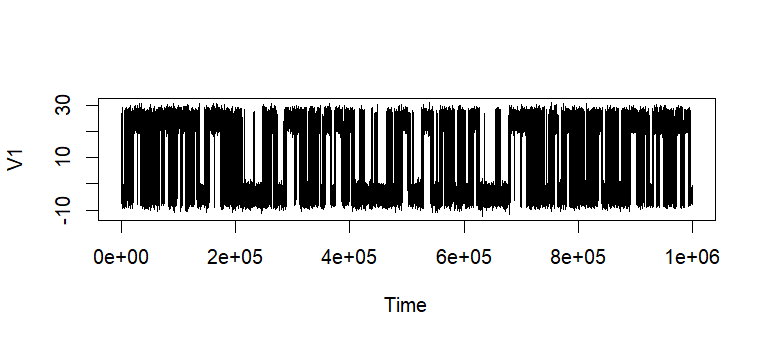
\includegraphics[width=5cm]{VR-reSGLD trace.png} }}%
    \qquad
    \subfloat[\centering Figure 2: SAGA-reSGLD trace.]{{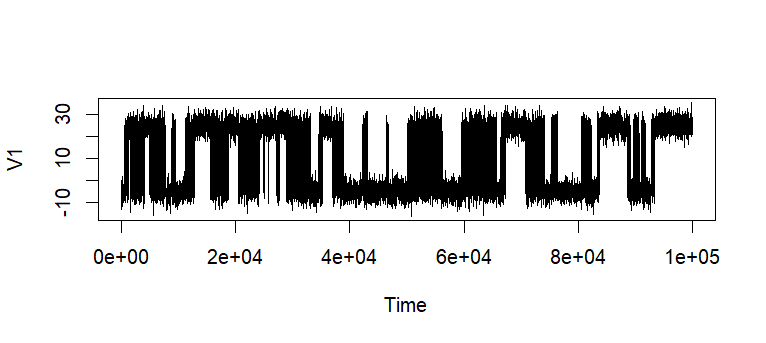
\includegraphics[width=5cm]{SAGA_plot.png} }}%
    \qquad
    \subfloat[\centering Figure 3: SAGA-reSGLD KDE.]{{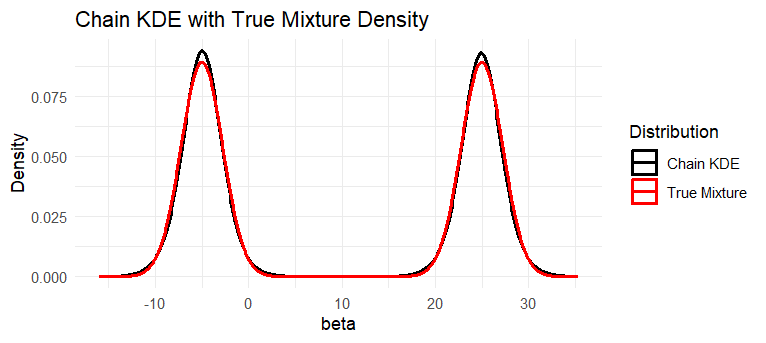
\includegraphics[width=5cm]{SAGA-KDE.png} }}%
    \label{fig:example}%
\end{figure}

Figure 1 shows the chain rapidly switches between the two modes of the posterior (one near $\beta\approx -5$ and the other near $\beta\approx 25$), indicating efficient exploration. VR-reSGLD’s control variate strategy for energy estimation enables frequent successful swaps between the low-temperature and high-temperature chains, thereby overcoming the metastability that a standard single-chain method would exhibit. In this example, VR-reSGLD fully recovers the two-mode structure of the target density and visits both modes regularly, whereas a conventional SGLD initialized near one mode would fail to escape that mode during the run. The ability to traverse between distant modes demonstrates the effectiveness of variance reduction in facilitating replica exchange.

Figure 2 shows frequent jumps between the two modes, similar to the VR-reSGLD performance in Figure 1. Initially, with untuned parameters, the SAGA-reSGLD chain was often stuck in one mode (resulting in a flat trace over long stretches), but after tuning, the swap acceptance rate increased substantially. The SAGA approach yields an equally rich exploration of the posterior modes, confirming that the SAGA-based variance reduction provides the same benefit of enabling mode-switching as the VR-reSGLD method. Notably, SAGA-reSGLD achieves this performance while using a much smaller minibatch (only $2\%$ of the data per iteration), demonstrating a significant improvement in per-iteration computational efficiency.

Figure 3 shows how The KDE from SAGA-reSGLD (solid blue curve) captures both prominent modes of the posterior—one near $\beta \approx -5$ and one near $\beta \approx 25$—with relative heights closely matching the expected 50/50 mixture. This aligns with the results reported for VR-reSGLD, which was shown to recover the true posterior density accurately. In our experiments, the SAGA-reSGLD estimator produces virtually the same two-mode density estimate as VR-reSGLD (and as the ground truth obtained by a long-run exhaustive sampler), indicating that the variance-reduced energy estimator does not introduce any bias. The densities are much more accurate than those from a single-chain SGLD, which would only reflect one mode. Both variance-reduced methods (VR-reSGLD and SAGA-reSGLD) achieve reliable uncertainty quantification for this multimodal posterior.
\newpage
In both Figure 1 and Figure 2, we see that the replica exchange procedure, aided by variance reduction, allows the cold-temperature chain to move between the two distant modes frequently. Quantitatively, the SAGA-reSGLD algorithm achieved a swap acceptance rate on par with VR-reSGLD in this experiment, with on the order of $10^4$ swaps in $10^6$ iterations (whereas a standard reSGLD without variance reduction yielded virtually no swaps without using an extremely large correction factor). The effective sample size (ESS) of the samples from the cold chain was markedly improved by these frequent swaps. For instance, considering $\beta$ as the parameter of interest, the ESS after a fixed number of iterations was significantly higher for SAGA-reSGLD than for a baseline reSGLD, meaning the SAGA-based chain produced more independent posterior samples in the same runtime. This is a direct consequence of better mixing between modes. We also note that SAGA-reSGLD does not require periodic full-data energy computations as in VR-reSGLD’s control variate update every $m$ iterations. This elimination of the global update step leads to practical speed-ups. In our implementation, SAGA-reSGLD used only 200 data points per iteration (versus 10,000 in VR-reSGLD) to maintain a stable swap acceptance probability, thereby reducing the computational cost per iteration by a factor of 50. Over the course of the run, this resulted in a substantial reduction in total data processing while attaining comparable accuracy in posterior estimates.

The theoretical justification for using SAGA in this context lies in its ability to provide an unbiased variance-reduced estimator. By continuously integrating new information into the stored energy values, the SAGA estimator $\tilde{L}^{(h)}$ remains much closer to the true full-data energy $L(\beta^{(h)})$ than a naïve minibatch estimate would be. In effect, after an initial pass through the data to initialize $E_i^{(h)}$, each subsequent iteration makes only a small adjustment to the global energy estimate. This yields an energy difference $\tilde{L}^{(1)} - \tilde{L}^{(2)}$ with low variance, similar to what would be obtained by using the entire dataset or a very large batch. Consequently, the correction term in the swap acceptance (which is proportional to the variance $\hat{\sigma}^2$) remains small, and the acceptance probability $S$ is closer to the ideal exchange probability one would get with exact energies. The improved swap rate fosters better equilibrium between the chains, allowing the cold chain to sample from multiple modes as if it had more time to explore or as if a tempered approach was used without penalty.

In terms of practical benefits, the SAGA-reSGLD approach offers a trade-off: it uses additional memory to store per-sample energies (on the order of $N$ values for each replica), but this investment yields more efficient sampling. Memory, in some cases, can generally be considered cheaper than computation in modern settings, so for moderately large $N$, storing a few extra vectors is feasible. The gain is that we avoid an expensive periodic recalculation of the full energy on all $N$ data points. In our experiments, the chosen update frequency of VR-reSGLD ($m=40$ in the setup of Deng et al.) meant a full pass through the data every 40 iterations, while SAGA-reSGLD required only the initial full pass and then updated a small fraction of the data each iteration. Thus, in scenarios where data is plentiful and iteration count needs to be high, SAGA-style variance reduction can substantially reduce the total computational burden. At the same time, SAGA’s continuous updates avoids the need to tune an update interval $m$ (which in VR-reSGLD presents a trade-off between variance reduction and computation cost). By effectively setting $m=1$ (updating parts of the control variate on every iteration), SAGA-reSGLD maximizes variance reduction at the cost of storing past energies.

Overall, our results demonstrate that integrating SAGA into the reSGLD framework inherits the theoretical advantages of variance reduction; namely, higher swap efficiency and faster convergence—while delivering practical improvements in computational efficiency. The SAGA-reSGLD algorithm was able to almost match the performance of VR-reSGLD on a challenging multimodal example, successfully reproducing the posterior distribution and mode-switching behavior, but with significantly less computational overhead per iteration. This suggests that SAGA-based variance reduction is a promising avenue for scaling up replica exchange MCMC methods in Bayesian deep learning and other big-data applications where both mixing and speed are crucial.

\newpage

\section{Conclusion}
We have introduced SAGA-reSGLD, a replica exchange SGLD algorithm that employs SAGA-style variance reduction for the energy estimators used in replica swap steps. Theoretically, reducing the variance of noisy energy differences leads to swap acceptance probabilities closer to those with exact energies, thus enabling more frequent exchanges and faster mixing between modes. Practically, our SAGA-based approach achieves this variance reduction without the need for large minibatches or frequent full-data computations, in contrast to previous VR-reSGLD implementations. Through experiments on a bimodal Gaussian mixture posterior, we showed that SAGA-reSGLD can efficiently explore a multimodal landscape, yielding accurate posterior density estimates and high effective sample sizes. It combines the strengths of variance reduction (improved convergence and sampling efficiency) with computational scalability (smaller batch sizes and no periodic global recalculation), albeit at the cost of additional memory usage.

Despite this, I acknowledge that this paper has it's limitations. They maily arise from my testing solely on the toy example and this algorithm having not been applied to a real data set (such as the CIFAR10 and CIFAR100 \cite{deng2021acceleratingconvergencereplicaexchange}). Future work may explore applying SAGA-reSGLD to higher-dimensional or real-world Bayesian inference problems, investigating its performance relative to other control variate techniques, and examining ways to mitigate the memory overhead (for instance, by subsampling the memory for extremely large $N$).

In summary, integrating the SAGA algorithm into the reSGLD framework provides a theoretically sound and empirically effective solution for sampling from complex posteriors. The SAGA-reSGLD algorithm retains the unbiasedness of the underlying MCMC and does not introduce noticeable bias in practice, as evidenced by its correct recovery of a known target distribution. I believe that variance-reduced energy estimation is a key component for accelerating convergence in stochastic gradient MCMC, and SAGA-reSGLD is a step toward more efficient and scalable Bayesian computation.

\newpage
\bibliographystyle{unsrt}   
\bibliography{references}
\end{document}
